%!TEX root = ../main.tex

\chapter{System Architecture}
\label{chp:architecture}

As discussed in Chapter \ref{chp:related}, there exist no off-the-shelf solution implementing the \ac{OBDF} paradigm. This implies that for the specific task of dealing with clinical and genomics data, it is necessary to design a system architecture, choosing components in such a way that the whole architecture results in being solid, privacy-oriented (with strong logging capabilities), and being capable to manage genomics data.
This chapter will firstly discuss the overall proposed architecture, that retraces the one presented in previous chapters. Subsequently, each layer will be presented in details, outlining how each components have been configured, reporting eventual code snippets. In order to better describe the source heterogeneity of data that may occur in contexts such as clinical and genomics, available relational data have been distributed among different sources.

\section{System Architecture Design}
\begin{figure}[ht]
    \centering
    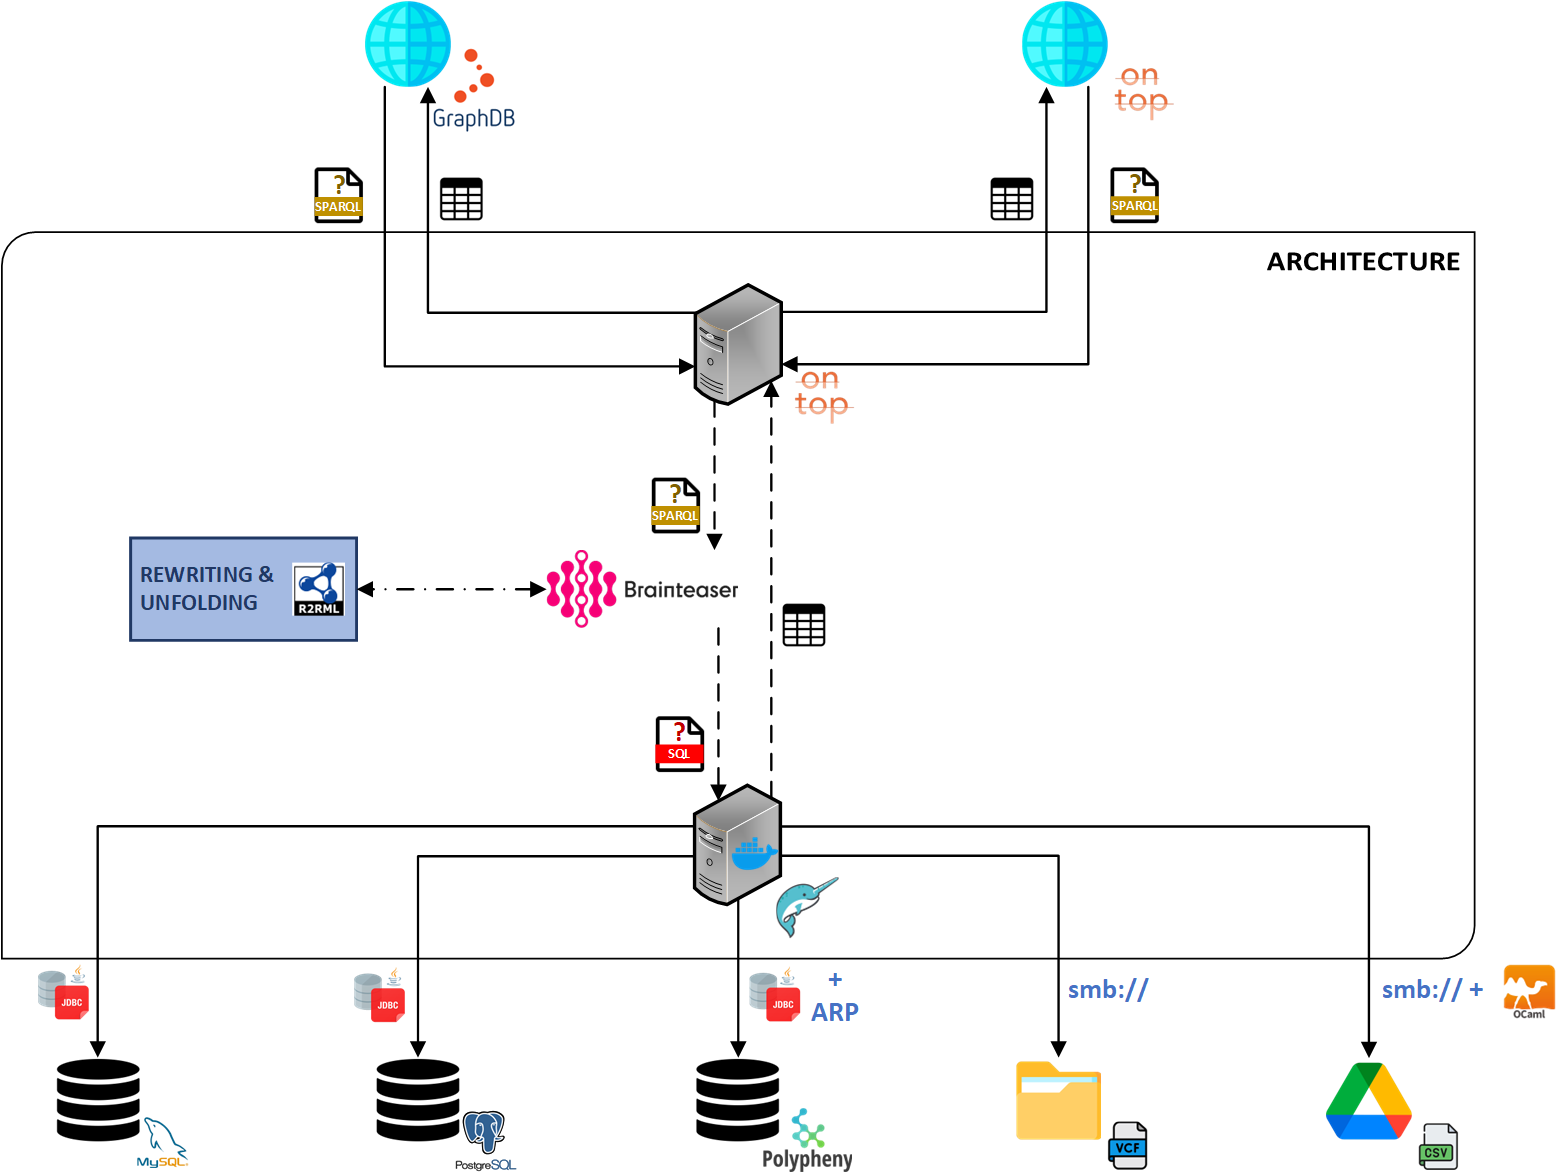
\includegraphics[width=14cm]{res/Drawing1.png}
    \caption{Proposed System Architecture}
    \label{fig:mirco_arch}
\end{figure}
The proposed architecture described in Fig. \ref{fig:mirco_arch} implements the \ac{OBDF} framework. It adopts Ontop as its semantic data integration layer and Dremio as its data federation layer. 

Briefly, Ontop have been chosen because it natively supports two high level mapping languages, that gives more freedom on their optimization, without the need to appeal to low level \ac{DL} languages, it is open-source and well maintained by the Free University of Bolzano data integration team, it comes embedded in GraphDB that offers solid \ac{API}s, and it comes even with an embedded web endpoint.

Dremio have been chosen as the virtualization and federation layer because, as discussed in the Chapter \ref{chp:background}, it is an open-source, robust and scalable software influenced both from its enterprise nature and from a consistent community providing contributions. Moreover, within its installation methods, it is possible to set it up through a Docker image: this may set the basis for the architecture packaging, expanding the image to other software components.

The semantic integration requires an ontology well describing the domain of clinical and genomics data. Considering the reusability principle that stands at the basis of the semantic web, we identified the Brainteaser ontology\footnote{https://brainteaser.dei.unipd.it/ontology/} as suitable for accomplishing this task. 

\section{Data Sources}
Given the relational nature of available data, we distributed it among five different platforms, so to exploit the federation capabilities of the data federation layer. The choice of the sources has been guided also by surveying commonly used ones in the biomedicine field in contexts like research and hospital diagnostic. As we will discuss, they encompasses more structured \ac{DBMS}s as well as simple \ac{CSV} files. We also included a novel \ac{DBMS} system, so to investigate how new, unknown data sources can be federated as soon as they figure out.

\subsection{MySQL}
MySQL\footnote{https://www.mysql.com/it/} is one of the most widely used relational \ac{DBMS} (DBMS) in the world. It is a \ac{FOSS} solution now distributed by Oracle\footnote{https://www.oracle.com/it/}. It is extensively employed across a variety of applications, from small personal projects to critical enterprise environments. In our system architecture, we've chosen MySQL considering its extensive adoption, possibly also in application softwares used in clinics and hospitals to collect patients data. 
In our environment, MySQL's role is to store part of the structured clinical data presented in Chapter \ref{chp:context}. 
The interfacing between MySQL and our data federation layer, Dremio, is performed through MySQL's JDBC connector. This setup allows Dremio to access and query MySQL data seamlessly.
No special modifications or configurations were required to integrate MySQL with Dremio, thanks to Dremio's native support for MySQL. We simply established a new data source within Dremio by specifying the connection parameters.

\subsection{PostgreSQL}
PostgreSQL\footnote{https://www.postgresql.org/} stands out as a widely adopted open-source relational \ac{DBMS}. It is particularly adopted within the research community due to its robustness, advanced features, and strong compliance with SQL standards. Many research institutions and academics prefer PostgreSQL for its extensive capabilities in managing complex data types and its support for sophisticated data manipulation operations. We considered PostgreSQL eligible to be a data source due to its common adoption in research contexts as a data collector.
Again, PostgreSQL's role in our environment is to store another portion of the structured clinical data presented in Chapter \ref{chp:context}.
Just like with MySQL, integrating PostgreSQL with Dremio did not require any specific modifications or additional configurations.

\subsection{Polypheny}